\section{Lineare Spannungsregler}

\subsection{Spannungsstabilisierung mit Z-Diode und BJT}

\begin{minipage}[c]{0.25\columnwidth}
    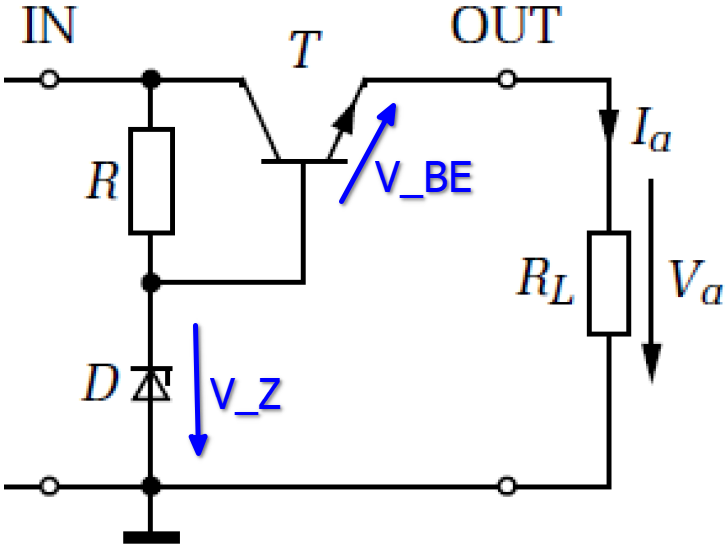
\includegraphics[width=\columnwidth]{images/spannungsstabilisierung_z-diode_bjt.png}
\end{minipage}
\hfill
\begin{minipage}[c]{0.72\columnwidth}
    $$ \boxed{ V_{out} = V_Z - V_{BE}} $$
    \begin{itemize}
        \item Ausgang kann viel Strom liefern
        \item Ausgangsspannung \textbf{sinkt} um ca. $20 \, \milli \volt$ bei \textbf{Verdoppelung} des Stroms
        \item Ausgangsspannung \textbf{sinkt} um $- 2 \frac{\milli \volt}{\kelvin}$
        \item \textbf{Keine Regelung} der Ausgangsspannung
        \item Schnell und stabil, aber nicht genau 
    \end{itemize}
\end{minipage}


\subsection{Linearer Spannungsregler}

\begin{minipage}[c]{0.3\columnwidth}
    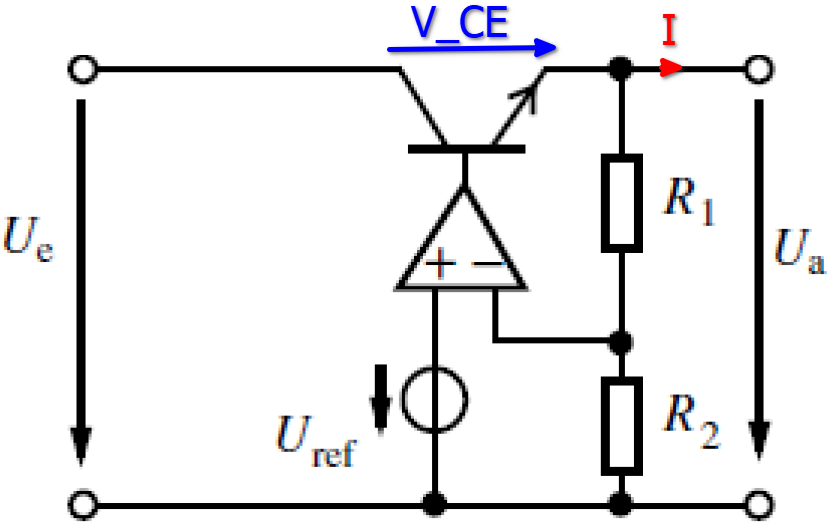
\includegraphics[width=\columnwidth]{images/linearer_spannungsregler.png}
\end{minipage}
\hfill
\begin{minipage}[c]{0.68\columnwidth}
    \begin{tabular}{c c}
        $ \boxed{ V_a = V_{ref} \Big( 1 + \frac{R_1}{R_2} \Big) } $ & $ \boxed{ P_V = V_{CE} \cdot I} $
    \end{tabular}
    \begin{itemize}
        \item OpAmp Ausgang ändert so lange, bis für die Spannungen gilt: $V_{R2} = V_{ref} \, (=1.25 \, \volt)$
        \item Minimaler Spannungsabfall $V_{CE}$ über Regler: bis $2.5 \, \volt$
        \item Regler kann sehr warm werden \textrightarrow\ Verlustleistung $P_V$
    \end{itemize}
\end{minipage}


\subsection{Low-Dropout-Regler mit pnp-Längstransistor (LDO)}

\begin{minipage}[c]{0.3\columnwidth}
    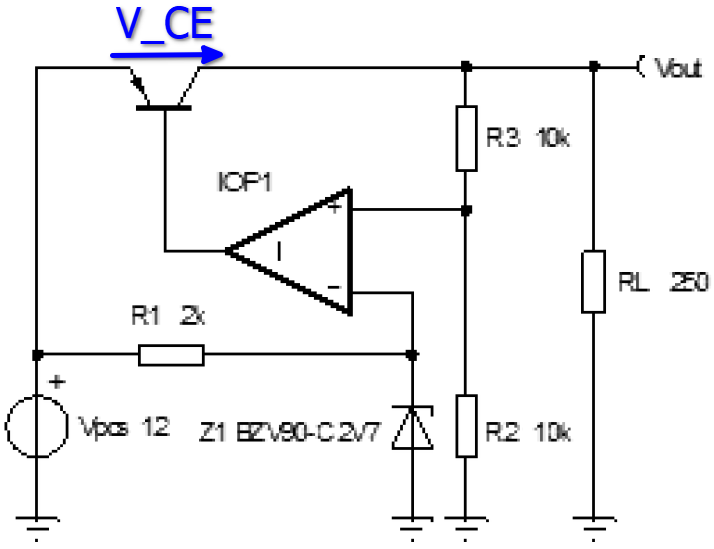
\includegraphics[width=\columnwidth]{images/ldo_pnp_transistor.png}
\end{minipage}
\hfill
\begin{minipage}[c]{0.68\columnwidth}
    \begin{itemize}
        \item Feedback auf \textbf{positiven} OpAmp-Eingang!
        \item Ansteuerung Längstransistor mit Basisspannung $< V_{out}$
        \item Kleiner minimaler Spannungsabfall $V_{CE}$ über Regler $(V_{CE,sat}$)
        \item Auch erhältlich mit PMOS-Transistor statt pnp-Transistor \textrightarrow\ Dropout-Spannung über Regler (PMOS) ist dann 
            abhängig vom Laststrom (PMOS $=$ gesteuerter Widerstand)
    \end{itemize}
\end{minipage}


\subsection{Einstellbarer Serie-Spannungsregler}

\begin{minipage}[c]{0.22\columnwidth}
    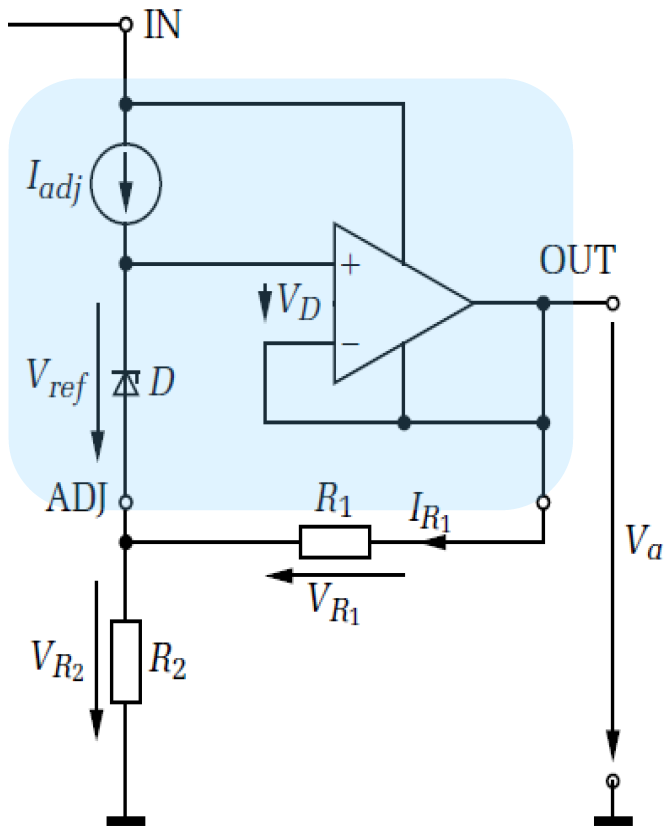
\includegraphics[width=\columnwidth]{images/einstellbarer_seriespannungsregler.png}
\end{minipage}
\hfill
\begin{minipage}[c]{0.76\columnwidth}
    % $$ \boxed{ \text{Für } I_{adj} \ll I_{R1}: \quad V_a = V_{ref} \cdot \Big( 1 + \frac{R_2}{R_1} \Big) }$$
    $$ \boxed{ V_a = V_{ref} \cdot \Big( 1 + \frac{R_2}{R_1} \Big) + I_{adj} \cdot R_2 }$$
    \begin{itemize}
        \item Widerstände $R_1$ und $R_2$ sind \textbf{extern} beschaltet!
        \item Interne Referenz: $V_{ref} = 1.25 \, \volt$ (Bandgap)
        \item OpAmp regelt, damit $V_{R1} = V_{ref}$
        \item Damit wird $V_{R2} = V_{ref} \cdot \frac{R_2}{R_1} + I_{adj} \cdot R_2$
    \end{itemize}
\end{minipage}
